\chapter{Concetti di base}

\section*{Introduzione}
Qui illustriamo alcuni dei concetti di base che serviranno per comprendere il resto della discussione, daremo una definizione di ontologia e tesauro, descriveremo brevemente gli strumenti utilizzati e i linguaggi con cui si descrivono le basi di conoscenza che tratteremo.


\section{Basi di conoscenza}
Le basi di conoscenza sono 
\subsection{Ontologie}
\subsubsection{Definizione}
In accordo con una definizione ampiamente accettata \cite{hitzler2021review} un'ontologia ha lo scopo di rappresentare un vocabolario per definire i concetti di un particoare dominio di interesse condiviso, ed è costituita da definizioni di classi, relazioni, funzioni e altri oggetti utili a rappresentare la conoscenza\cite{gruber1993translation}. 

La definizione è ancora un po' vaga, più precisamente un'ontologia è una base di conoscenza che permette di descrivere concetti e relazioni tra di essi specificando questi oggetti tramite un linguaggio di rappresentazione della conoscenza basato su una logica formale.
\subsubsection{Scopo delle ontologie}
Nel contesto del web semantico\footnote{Un'estensione del World Wide Web in cui le informazioni siano comprensibili ad un automa\cite{berners2001new}} le ontologie sono il mezzo principale per condividere, integrare e scoprire dati\cite{hitzler2021review}.
\subsubsection{Manipolare ontologie}
 Dato lo scopo delle ontologie risulta essere un argomento centrale la possibilità di riutilizzare, modificare e ampliare ontologie esistenti. Spesso le basi di conoscenza sono sì strutturate, ma sono eterogenee e non permettono interoperabilità. Scopo di questo lavoro è quello di presentare degli strumenti per manipolare basi di conoscenza (ci concentriamo si tesauri e ontologie) operando in modo tale da rendere compatibili informazioni tratte da fonti differenti. 
 
 Il testo \cite{suarez2015neon} presenta una trattazione teorica approfondita sulle metodologie per sviluppare un'ontologia, in particolare il framework NeOn prevede vari scenari tipici in cui ci si può trovare quando si voglia costruire un ontologia, si fa particolare attenzione ai casi nei quali siano già presenti informazioni, ma queste vanno riorganizzate.
\subsubsection{Esempio}
Consideriamo una semplice ontologia che rappresenta persone con legami di parentela genitore-figlio; le persone hanno uno o più nomi salvate nel tag \verb|comment|. Modelliamo questa ontologia con una classe \verb|Persone| e una sottoclasse \verb|Genitori| (i cui individui sono \verb|Persone| che realizzano la relazione \verb|genitoreDi|). Creiamo la relazione \verb|genitoreDi|. Infine popoliamo l'ontologia con alcuni individui. Il risultato ottenuto con Protégé è un documento XML di questo tipo:
\addxml{persone.rdf}{lst:persone.rdf}{Code/persone.rdf}
\begin{wrapfigure}{r}{0.5\textwidth}
	\centering
	\caption{Grafo dell'ontologia persone}
	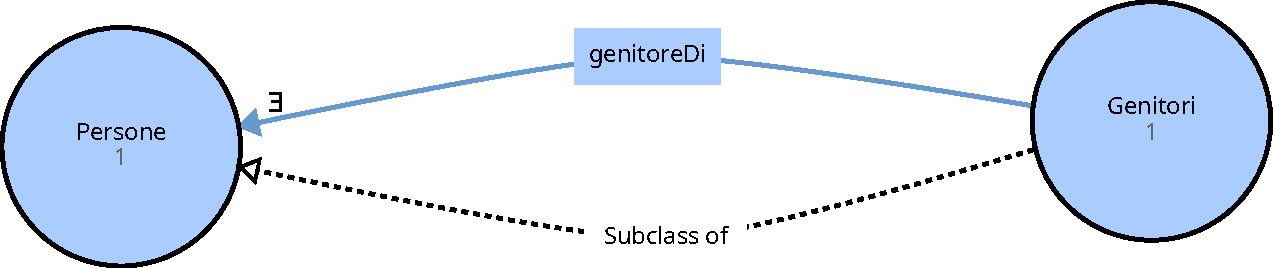
\includegraphics[width=0.5\textwidth]{Picture/persone.rdf.pdf}
\end{wrapfigure}

Per quanto non sia impossibile leggere la struttura e i dati dal listato precedente un modo naturale per rappresentare le ontologie è sotto forma di grafi. Qui vediamo il grafo\footnote{tutti i grafi presenti un questo elaborato sono stati ottenuti grazie a http://vowl.visualdataweb.org/webvowl.html} che mostra la struttura dell'ontologia e possiamo apprezzare quanto sia semplice la sua struttura rispetto a quello che avremmo potuto immaginare dal listato \ref{lst:persone.rdf}. Nel grafo non sono rappresentati gli individui, possiamo comunque leggere quanti ve ne sono per ogni classe (in questo caso un individuo di tipo \verb|Persone| e uno di tipo \verb|Genitori|)


\subsection{Tesauri}
Nella loro accezione più generale possibile i tesauri sono risorse nelle quali termini affini sono raggruppati assieme\cite{kilgarriff2000s}. In particolare un tesauro fornisce un vocabolario preciso e controllato rispetto ad un particolare dominio di interesse.\cite{srinivasan1992thesaurus} Queste strutture possono aiutare il ricercatore a riformulare le strategie di ricerca fornendo una serie di sinonimi, contrari, definizioni e traduzioni in altre lingue del termine cercato.

Esistono diversi tipi di tesauro in base alle modalità di costruzione e fruizione \cite{kilgarriff2000s}, nel nostro caso il tesauro sarà costituito da un vocabolario tassonomico in cui le relazioni tra oggetti sono di tipo BT (broader term), cioè ogni concetto può avere un riferimento ad un concetto più generale, formando in questo modo una struttura ad albero. 

Come si può immagina
\section{Strumenti di editing}

\subsection{Protégé}

\subsection{\cduce}
\cduce è un linguaggio di programmazione funzionale, staticamente tipato e orientato allo sviluppo di applicazioni che lavorano su documenti XML\cite{cduceLanguage}
\subsection{Feature}\label{fature_cduce}
\subsubsection{Pattern matching}
\label{CDucePattern}
È un'operazione fondamentale in \cduce ed ha la forma:
\begin{minted}[tabsize=2, breaklines, bgcolor=bg]{OCaml}
match e with
	| p1 -> e1
	...
	| pn -> en
\end{minted}
Si cerca di fare il match tra la valutazione di un'espressione \verb|e| e vari pattern \verb|pi|. Il primo pattern che fa il match con \verb|e| attiva la corrispondente espressione sulla destra che può usare le variabili legate dal pattern.


\section{Metalinguaggi}

\subsection{OWL}

\subsection{SKOS}
